



\section{Introduction}
Sur l'ensemble des 35 probl\`emes, apr\`es avoir modifi\'e \`a la main les codes g\'en\'er\'es, seuls deux probl\`emes ne donnent
pas une valeur de Hessien correcte par Tapenade. Nous allons voir dans ce chapitre le temps d'ex\'ecution 
des d\'eriv\'ees et allons v\'erifier que les bornes th\'eoriques de complexit\'e sont respect\'ees. 
Ensuite, nous \'etudierons les variantes de m\'ethodes de descente sur la librairie MGH.


\section{Temps de calcul des op\'erations critiques}
Nous allons commencer par \'etudier les op\'erations \'el\'ementaires pour v\'erifier que les m\'ethodes sont comparables.
Les tests ont \'et\'e effectu\'es sur des fonctions arbitrairement choisies.
% 


\subsection{D\'ecomposition fournie par Scilab}
\label{chap4:decomp}
Pour commencer, il est \`a noter que la r\'esolution 
des syst\`emes triangulaires dans scilab n'est g\'en\'eralement pas efficace. Il s'av\`ere que la d\'etection du syst\`eme triangulaire 
n'est pas faite syst\'ematiquement. La figure \ref{fig:lu} r\'ev\`ele que sur les quatre tests de r\'esolution
 $Lx=e$, $L'x=e$, $U'x=e$, $Ux=e$ o\`u $L$ et $U$ proviennent de la d\'ecomposition $LU$ r\'ealis\'e par scilab et
 $e=(1)_{1\leq i\leq n}$ un vecteur colonne, une seule est performante.

\begin{figure}
\caption{R\'esolution d'un syst\`eme triangulaire par scilab avec une d\'ecomposition LU, sur les quatre versions,
qu'une seule n'est efficace.}
\center
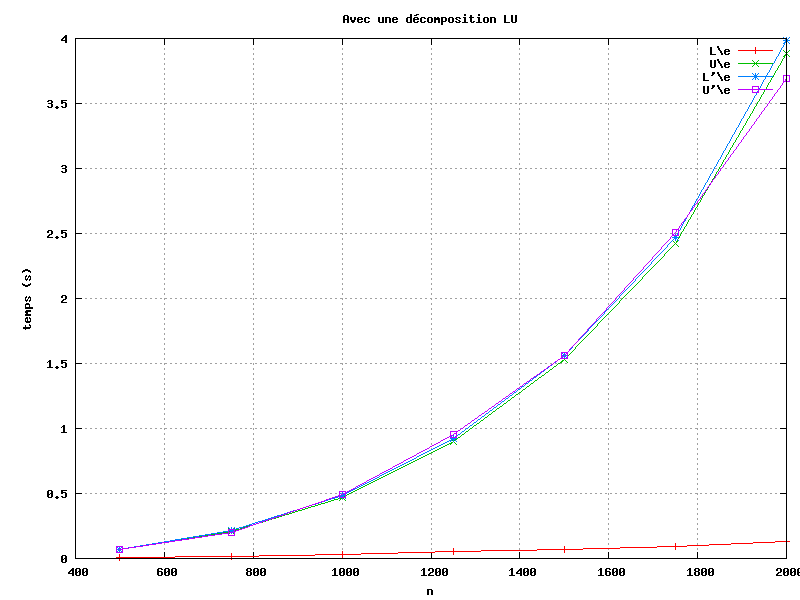
\includegraphics[scale=0.39]{figures/LU.png}
\label{fig:lu}
\end{figure}


\begin{figure}
\caption{R\'esolution d'un syst\`eme triangulaire par scilab avec une d\'ecomposition de Cholesky}
\center
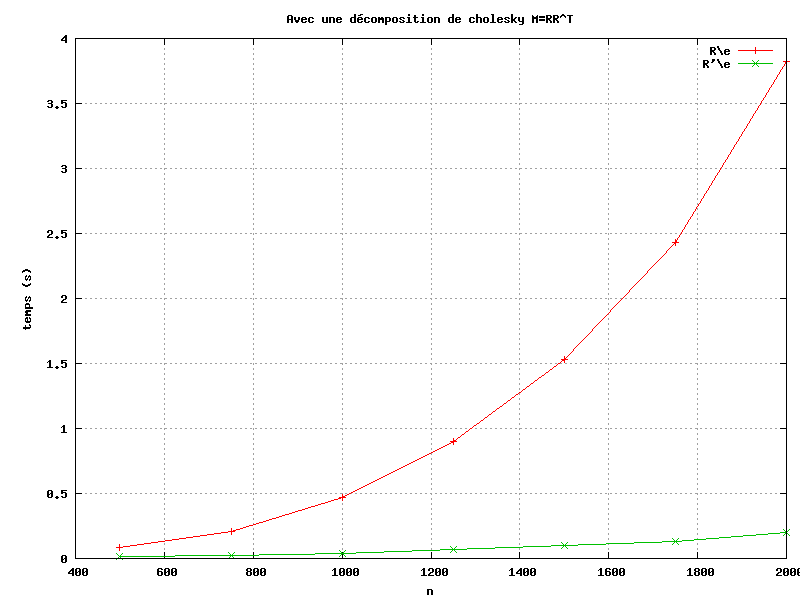
\includegraphics[scale=0.39]{figures/chol.png}
\label{fig:chol}
\end{figure}

C'est pour cette raison que nous avons pr\'ef\'er\'e choisir une d\'ecomposition \'ecrite en fortran pour nos calculs.


    \subsection{D\'eriv\'ees d'ordres divers}

% 
% Pour \'evaluer les temps de calcul de ces op\'erations critiques, j'ai utilis\'e les fonctions trigonom\'etrique et 
% chebyquad.
% 
% 
% \subsection{Matrices creuses}
\'Etant donn\'e que nous voulons faire des tests de calcul sur des fonctions types, il est pertinent
d'\'etudier le comportement des fonctions et notamment si la matrice hessienne est creuse.
La figure \ref{fig:trigo} indique par des points les \'el\'ements non nuls de la matrice hessienne
pour la fonction trigonom\'etrique.
On n'exploite pas le fait que la matrice soit creuse mais les coûts de calculs seront probablement
diminu\'es quand même car les op\'erations seront faites sur des z\'eros.



% \begin{figure}
% \caption{Matrice hessienne de la fonction disc\`ete \`a valeurs finies (28)}
% \center
% 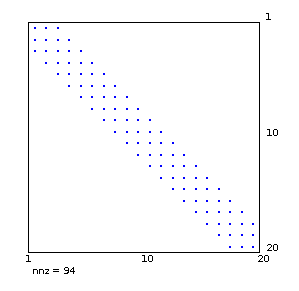
\includegraphics[scale=0.7]{figures/bound.png}
% \label{fig:bound}
% \end{figure}
% 
Nous allons pr\'esenter trois exemples de fonction appartenant \`a la librairie; la fonction bien connue en optimisation Rosenbrock, g\'en\'eralis\'ee \`a dimension variable, 
une fonction trigonom\'etrique et une fonction utilisant les polynômes de Chebychev.
% 
% 
% 
% Comme les polynômes sont de plus en plus compliqu\'es \`a calculer quand la dimension augmente, le coût de $f$
% ne va pas être lin\'eaire par rapport \`a $n$.



\paragraph{Fonction trigonom\'etrique}
\begin{align*}
% \begin{equation}
n \text{ variable, } m=n \\
f_i(x)=n-\sum_{j=1}^{n}cos(x_j)+i(1-cos(x_i))-sin(x_i) \\
x_0= [1/n, \cdots , 1/n] \\
min_x f(x) = 0
% \end{equation}
\end{align*}

% \begin{figure}
% \caption{Matrice hessienne de la fonction trigonom\'etrique}
% \center
% 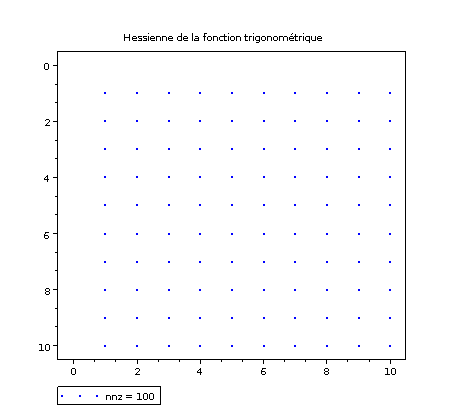
\includegraphics[scale=0.4]{figures/trigo.png}
% \label{fig:trigo}
% \end{figure}


\begin{figure}
\caption{Matrice hessienne de la fonction trigonom\'etrique, les points bleus repr\'esentent les \'el\'ements non nuls de la
matrice.}

\begin{center}
\fbox{
\begin{minipage}[c]{0.335\textwidth}
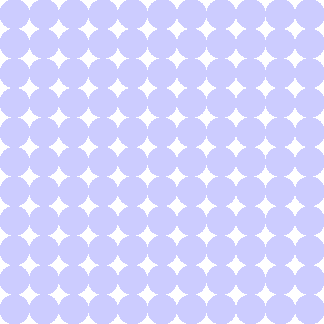
\includegraphics[scale=1]{figures/figure_16}
\end{minipage}
}
\end{center}
\label{fig:trigo}
\end{figure}






La matrice hessienne de la fonction trigonom\'etrique est une matrice pleine \ref{fig:trigo}, cette fonction pourra nous servir 
de r\'ef\'erence car les calculs sont relativement simples.



% \subsection{Fonction Rosenbrock \'etendue}
\paragraph{Fonction Rosenbrock \'etendue}

\begin{align*}
n\text{ variable mais pair } m=2 \\
f_{2i-1}(x)=10(x_{2i}-x^2_{i-1})\\
f_{2i}(x)=1-x_{2i-1}\\
x_0= (\xi_i) \text{ o\`u } \xi_{2i-1}= -1.2  \text{ et } \xi_{2i}=1 \\
min_x f(x) = 0 \text{ en } [1,\cdots ,1]
\end{align*}

Chaque composante de la fonction n'est d\'ependante que de deux variables, c'est pourquoi la matrice hessienne est creuse.

\begin{figure}
\caption{Matrice hessienne de la fonction de Rosenbrock \'etendue}
\begin{center}
\fbox{
\begin{minipage}[c]{0.335\textwidth}
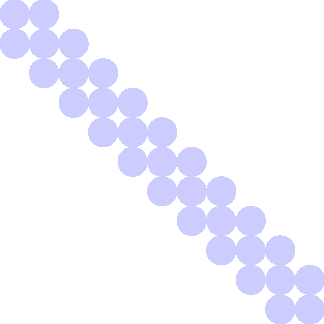
\includegraphics[scale=1]{figures/figure_17}
\end{minipage}
}
\end{center}
\label{fig:rosenbrock}
\end{figure}



% \begin{figure}
% \caption{Newton - La recherche lin\'eaire restreint \`a fournir des it\'er\'es dont la valeur de l'objectif est 
% toujours d\'ecroissante tandis que sans recherche, on s'\'eloigne pour converger plus vite.}
% \begin{center}
% \fbox{
% \begin{minipage}[c]{0.6\textwidth}
% 
% \end{minipage}
% }
% \end{center}
% \label{fig:Newton}
% \end{figure}



















La fonction a \'et\'e propos\'ee par Rosenbrock en 1960 afin de comparer des algorithmes de descente. Dans 
le cas avec $n=2$, la fonction forme un sillon \'etroit, ce qui oblige les m\'ethodes de descente \`a suivre une courbe. 
L'agorithme du gradient par exemple est tr\`es m\'ediocre car il "rebondit" sur chaque parois sans avancer vraiment.
En ce qui concerne la m\'ethode de Newton, augmenter la dimension de la fonction n'influencera pas le nombre d'it\'erations
car le probl\`eme pourra être vu comme $\frac{n}{2}$ probl\`emes de Rosenbrock qui s'effectuent parall\`element.








\begin{figure}[h]
\caption{Alogrithme du gradient sur Rosenbrock : 19436 it\'erations}
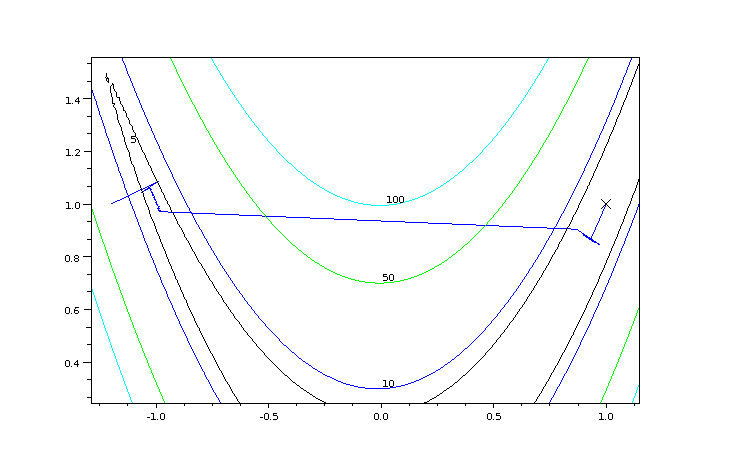
\includegraphics[scale=0.3]{figures/gradient.png}
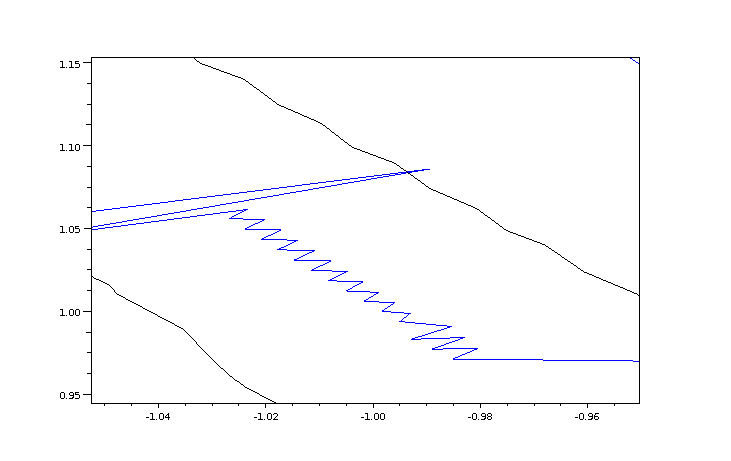
\includegraphics[scale=0.3]{figures/gradientzoom.png}
\end{figure}




% \subsection{Fonction Chebyquad}
\paragraph{Fonction Chebyquad}

\begin{align*}
n \text{ variable, } m=n \\
f_i(x)=\frac{1}{n}\sum_{j=1}^{n}T_i(x_j)-\int_0^1 \! T_i(x)dx \\
\text{O\`u }T_i\text{ est le i\`eme polynôme de Chebychev r\'eduit \`a l'intervale } [0,\ 1] \\
\int_0^1 \! T_i(x)dx= 0 \text{ pour i paire}\\
\int_0^1 \! T_i(x)dx= \frac{-1}{i^2-1} \text{ pour i impaire}\\
x_0= (\xi_j) \text{ o\`u } \xi_j=j/(n+1)\\
f=0 \text{ pour } m=n \text{,}\ 1\leq n\leq 7\ \text{ et }\ n=9\\
f=3.51687... 10^{-3}\ \text{ pour }\ n=m=8 \\
f=6.50395... 10^{-3}\ \text{ pour }\ n=m=10 \\
\end{align*}



% \begin{figure}
% \caption{Matrice hessienne de la fonction de Chebyquad}
% \center
% 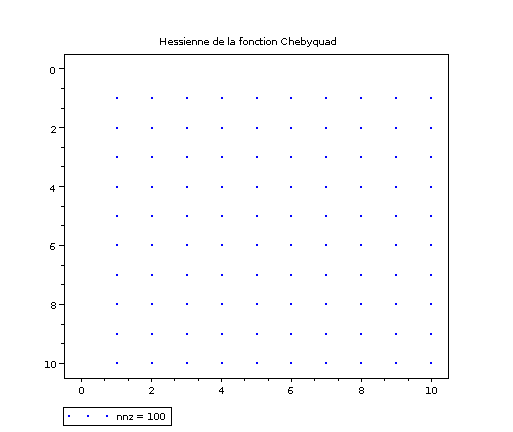
\includegraphics[scale=0.4]{figures/chebyquad.png}
% \label{fig:chebyquad}
% \end{figure}

\begin{figure}
\caption{Matrice hessienne de la fonction de Chebyquad}
\begin{center}
\fbox{
\begin{minipage}[c]{0.335\textwidth}
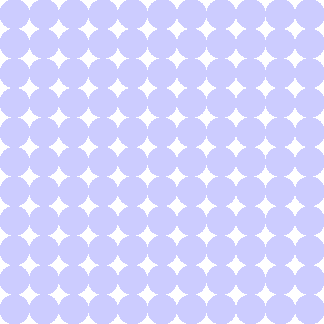
\includegraphics[scale=1]{figures/figure_16}
\end{minipage}
}
\end{center}
\label{fig:chebyquad}
\end{figure}




Ces trois fonctions ont des dimensions variables ; elle refl\`etent l'ensemble des r\'esultats qui sont \'equivalents pour les calculs des d\'eriv\'ees.
La fonction Chebyquad est plus particuli\`ere dans le sens o\`u le temps d'ex\'ecution de la fonction n'est pas proportionnel
\`a la dimension car les polynômes sont de plus en plus complexes \`a calculer en fonction de $n$. 





\paragraph{Gradient recod\'e vs gradient fourni par la routine}
 Pour la fonction trigonom\'etrique, comme le montre \ref{fig:temps14},
 le calcul du gradient donn\'e par la routine de netlib n'est pas 
efficace. Ceci s'explique par le fait que pour l'obtenir, on utilise la relation $$ \nabla f(x)=F(x)^T\nabla F(x)$$ en notant que 
$$f(x)= \frac{1}{2}\sum_{i=1}^{m}F_i(x)^2$$
Le calcul de la Jacobienne $\nabla F(x)$ de taille $n$ par $m$ impose beaucoup de calculs qui peuvent être \'evit\'es.
En recodant le gradient de la fonction, les multiplications sur les lignes sont factorisables, on am\'eliore nettement 
l'ex\'ecution.

\begin{figure}
\caption{Temps d'\'evaluation du gradient en modifiant la taille
de $x$ et celui du gradient recod\'e}
\center
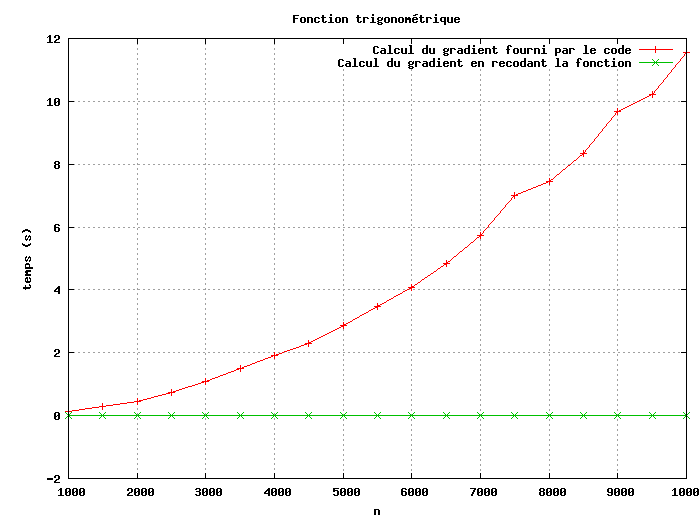
\includegraphics[scale=0.4]{figures/temps14.png}
\label{fig:temps14}
\end{figure}


% \begin{figure}
% \caption{Gradient de la fonction trigonom\'etrique dont le code \`a \'et\'e am\'elior\'e comparativement \`a celui d'origine}
% \center
% 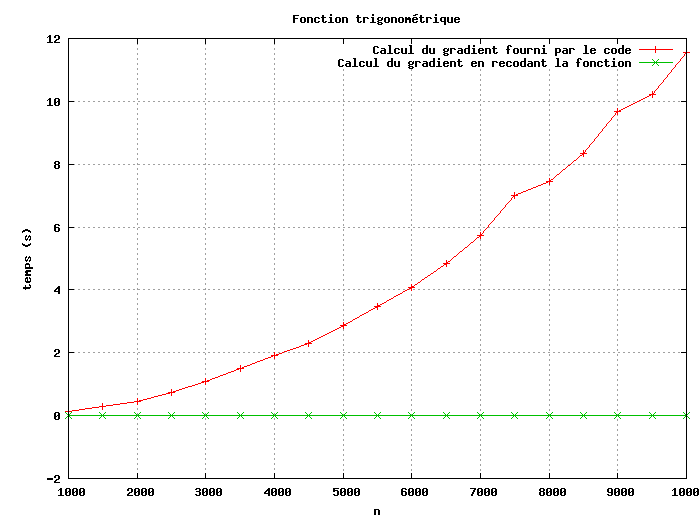
\includegraphics[scale=0.4]{figures/temps14.png}
% \label{fig:temps14}
% \end{figure}




% Avec le code g\'en\'er\'e par tapenade :
% Tableau pour calculer $f(x)$, $\nabla f(x)$,$\nabla^2 f(x)$, $\nabla f(x).v$, $\nabla^2 f(x).uv$






\paragraph{Fonction et mode inverse}

Afin de pouvoir comparer les temps d'ex\'ecution de la fonction et du mode inverse, les appels sont faits
plusieurs fois dans une boucle de mille it\'erations. En effet, même pour une dimension de $n=10000$,
 le temps pour \'evaluer la fonction est inf\'erieur au pas d'horloge unitaire de $4$ms. On remarque sur la
 figure \ref{fig:temps2} que l'obtention du gradient par le mode
inverse est clairement proportionnel au coût de la fonction avec un facteur de proportionnalit\'e d'environ
deux; pour rappel, la borne th\'eorique est de quatre. Le mode inverse est nettement plus performant qu'une implantation na\"ive.


\begin{figure}
\caption{Temps de calcul de la fonction et du gradient en mode direct par Tapenade dans une boucle de mille it\'erations, fonction trigonom\'etrique}
\center
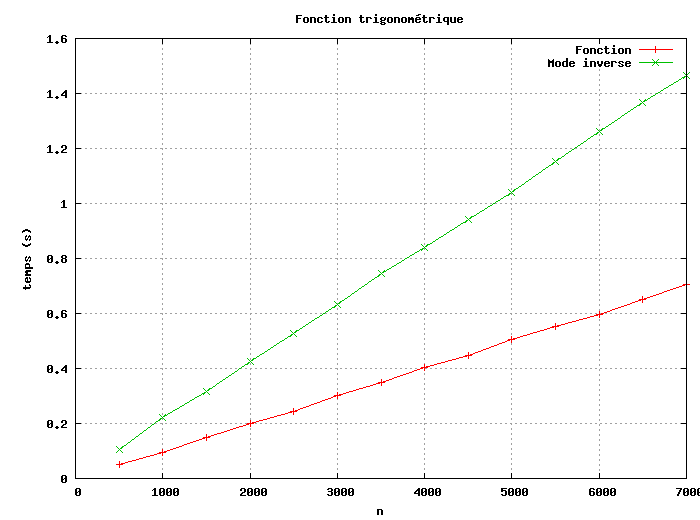
\includegraphics[scale=0.4]{figures/temps2.png}
\label{fig:temps2}
\end{figure}


La figure \ref{fig:temps6} montre que l'\'evaluation de la fonction Chebyquad n'est pas proportionnelle \`a la dimension; il ne s'agit pas d'une droite.
En revanche, le gradient ressemble \`a un facteur pr\`es \`a celle de l'\'evaluation. On peut observer que $\#(\nabla f)\simeq 3.5 \#(f)$.


\begin{figure}
\caption{Fonction chebyquad, mode inverse vs temps fonction, l'\'evaluation n'est pas proportionnelle \`a la dimension, par contre le gradient 
ressemble \`a un facteur pr\`es \`a $f$}
\center
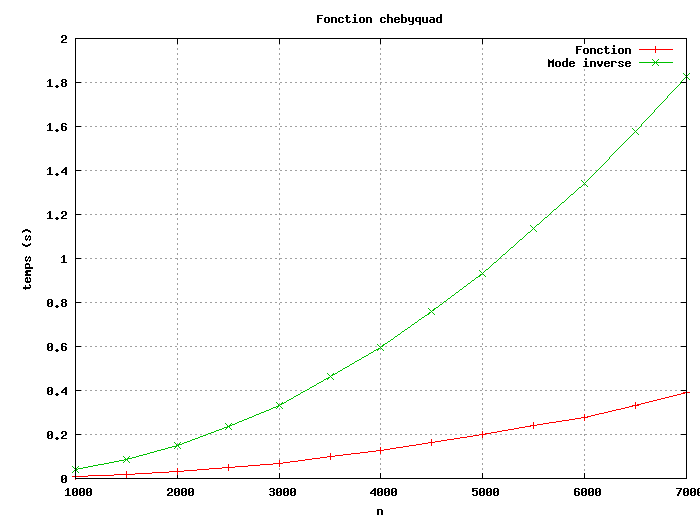
\includegraphics[scale=0.4]{figures/temps6.png}
\label{fig:temps6}
\end{figure}



\paragraph{Le mode multi-directionnel}
Le mode multi-directionnel correspond au mode direct appliqu\'e \`a chacune des composantes;
il \'equivaut \`a effectuer $\nabla f(x).(e_i)$ pour chaque $1\leq i\leq n$.



Dans la figure \ref{fig:temps1}, nous pouvons voir que le temps en mode multi-directionnel est
 environ le même que pour calculer le gradient par diff\'erences finies. Le mode multi-directionnel
n'est pas avantageux puisqu'il effectue le mode tangent $n$ fois.


\begin{figure}
\caption{Temps de calcul - fonction trigonom\'etrique}
\center
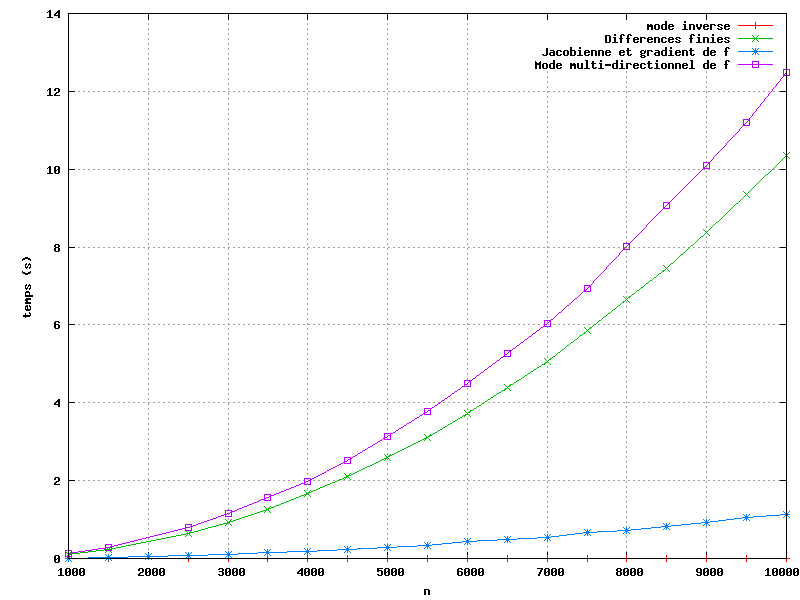
\includegraphics[scale=0.4]{figures/temps1.png}
\label{fig:temps1}
\end{figure}

\begin{figure}
\caption{Mode multi-directionnel : $\nabla f(x)$}
\center
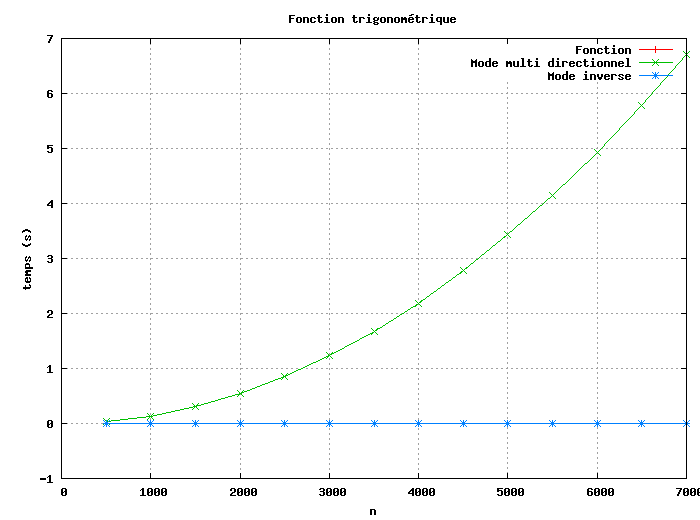
\includegraphics[scale=0.4]{figures/temps4.png}
\label{fig:temps4}
\end{figure}


\paragraph{Hessien$\times$vecteur}

Comme pour le mode inverse, le coût du hessien multipli\'e par un certain vecteur calcul\'e par mode direct sur mode inverse est proportionnel
 au coût de la foncion \ref{fig:temps3} environ 4$\times\#(f)$.


\begin{figure}
\caption{Mode tangent sur inverse (vert $\times$) sur une boucle de mille it\'erations, ce qui correspond au calcul de $\nabla^2 f(x).v$ pour un certain vecteur, le r\'esultat
est donc aussi un vecteur}
\center
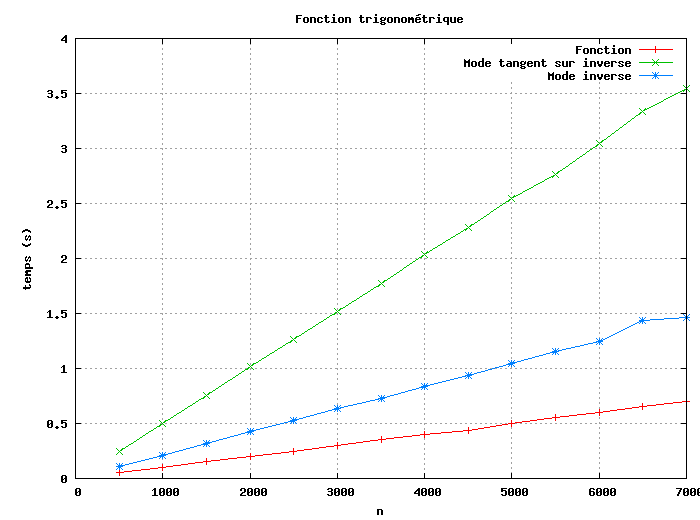
\includegraphics[scale=0.4]{figures/temps3.png}
\label{fig:temps3}
\end{figure}






\paragraph{Hessien}

Pour obtenir la matrice hessienne \ref{fig:temps16}, il faut appliquer le mode multi-directionnel qui n'est pas 
extrêmement performant sur le mode inverse. 


\begin{figure}
\caption{Mode multi-directionnel sur inverse (vert $\times$) ce qui donne la hessienne $\nabla^2 f(x)$ pour un certain vecteur, le r\'esultat
est donc aussi un vecteur}
\center
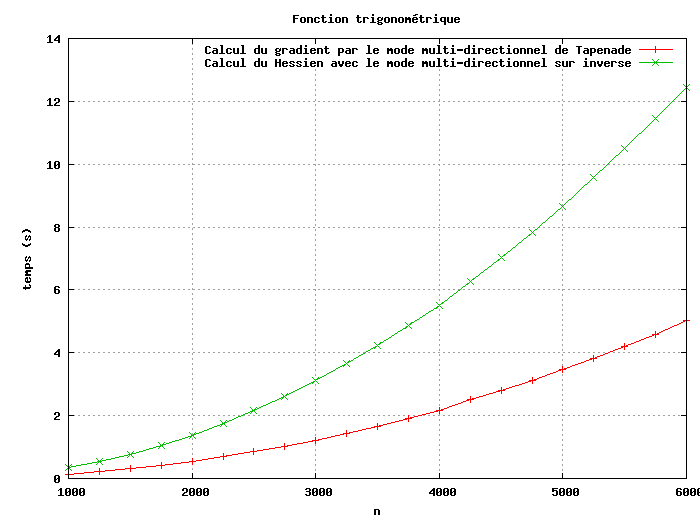
\includegraphics[scale=0.4]{figures/temps16.png}
\label{fig:temps16}
\end{figure}



\paragraph{Ordres sup\'erieurs}
Le coût des op\'erations $\nabla^3 f(x)\cdot u \cdot v$ et $\nabla^4f(x)\cdot u \cdot v \cdot w$ ne d\'ependent pas de $n$ comme le montre la figure
\ref{fig:temps17}. Toutes les courbes sont affines.

\begin{figure}
\caption{Temps des op\'erations  $\nabla^4f(x)\cdot u \cdot v \cdot w$ en vert et marron, $\nabla^3 f(x)\cdot u \cdot v$ en rouge : elles ne d\'ependent pas de $n$
et sont proportionnelles au coût de la fonction.}
\center
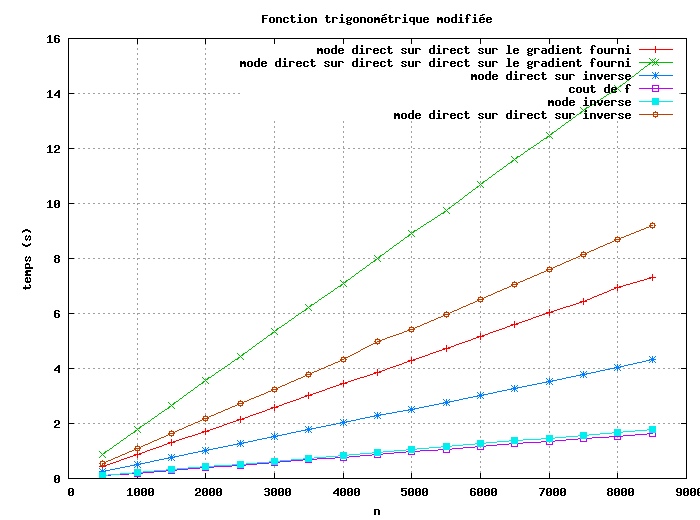
\includegraphics[scale=0.4]{figures/temps17.png}
\label{fig:temps17}
\end{figure}





\subsection{D\'ecomposition de Cholesky modifi\'ee et r\'esolution de syst\`eme lin\'eaire}


Comme le montre la figure \ref{fig:temps8}, la factorisation modifi\'ee est l'op\'eration qui prend le plus de temps,
elle a un comportement en $n^3$. La r\'esolution du syst\`eme lin\'eaire est plus rapide que le changement de la 
diagonale parce qu'elle est ex\'ecut\'ee en fortran.
\begin{figure}
\caption{R\'esolution du syst\`eme $Ax=b$ avec la factorisation de Cholesky modifi\'ee}
\center
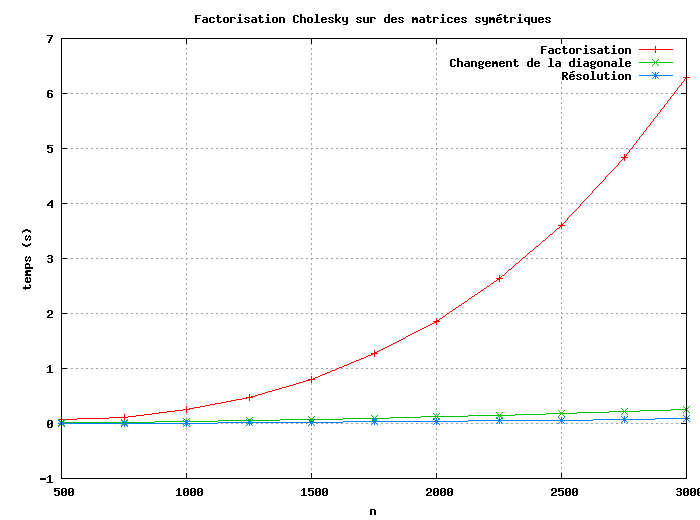
\includegraphics[scale=0.4]{figures/temps8.png}
\label{fig:temps8}
\end{figure}


\begin{table}[h]
	\begin{center}
\begin{tabular}{|c|c|c|c|c|}\hline
n & D\'ecomposition & Arrangement & R\'esolution & $A \backslash b$ avec Scilab\\
 & $A\leftarrow LDL^T$ & $D\leftarrow \Tilde{D}+\Delta \Tilde{D}$& $Lu=b$, $\Tilde{D}v=u$, $L^Tx=v$ & \\
\hline
$500 $&$  0.037000 $&$  0.011000 $&$ 0.002000 $&$ 0.090000$\\\hline
$750 $&$ 0.122000 $&$ 0.026000 $&$ 0.005000 $&$ 0.220000$\\\hline
$1000 $&$ 0.254000 $&$ 0.038000 $&$ 0.010000 $&$ 0.486000$\\\hline
$1250 $&$ 0.475000 $&$ 0.055000 $&$ 0.015000 $&$ 0.944000$\\\hline
$1500 $&$ 0.809000 $&$ 0.075000 $&$ 0.022000 $&$ 1.607000$\\\hline
$1750 $&$ 1.278000 $&$ 0.097000 $&$ 0.030000 $&$ 2.543000$\\\hline
$2000 $&$ 1.863000 $&$ 0.123000 $&$ 0.038000 $&$ 3.732000$\\\hline
$2250 $&$ 2.636000 $&$ 0.149000 $&$ 0.047000 $&$ 5.413000$\\\hline
$2500 $&$ 3.602000 $&$ 0.179000 $&$ 0.057000 $&$ 7.402000$\\\hline
$2750 $&$ 4.830000 $&$ 0.215000 $&$ 0.070000 $&$ 10.116000$\\\hline
$3000 $&$ 6.320000 $&$ 0.251000 $&$ 0.084000 $&$ 13.327000$\\\hline
\end{tabular}
	\end{center}
	\caption{Temps de calcul pour chaque \'etape de la r\'esolution du syst\`eme $Ax=b$, bien que la modification de la diagonale soit
$\mathcal{O}(n)$, elle est moins efficace que la r\'esolution car elle est cod\'ee en scilab.}
	\label{tab:newton}
\end{table}







\section{M\'ethode de descente avec recherche lin\'eaire}
Les m\'ethodes d'ordres sup\'erieurs requi\`erent souvent 
moins d'it\'erations. Nous pr\'esentons quelques exp\'eriences illustrant que notre implantation traduit cette r\'eduction du nombre
d'it\'erations dans une r\'eduction du temps de calcul. Les directions ont \'et\'e test\'ees avec et sans recherche lin\'eaire.
Il s'av\`ere que sans recherche lin\'eaire, les algorithmes n'aboutissent pas dans beaucoup de cas car $x_0$ est \'eloign\'e de la solution et
la direction peut être trop grande.
Pour les m\'ethodes de Newton et Chebychev, j'ai d'abord conserv\'e le point initial donn\'e dans les fonctions
de la librairie. Ce point est g\'en\'eralement assez proche de la solution. Dans le tableau, 
nous notons $x_{N_f}$ et $x_{C_f}$ les points finals des m\'ethodes de Newton et Chebychev respectivement. 
Cette norme confirme ou infirme le fait que les deux algorithmes convergent bien vers le même point.

On remarque sur la figure \ref{fig:vraies} que la m\'ethode de Chebychev comme celle d'extrapolation d'ordre trois,
 n'aboutit pas dans plusieurs cas, le maximum d'it\'erations \'etant fix\'e \`a $999$. Afin d'am\'eliorer ceci,
nous allons choisir la direction de Chebychev uniquement lorsqu'il s'agit bien d'une direction de descente.
 Dans le cas contraire nous reprendrons la direction de Newton.

% % Pourquoi n'est pas pertinent ?? On ne sais pas d\'ej\`a que les m\'ethodes convergent tr\`es mal 
% % a priori nous avons pas besoin de direction de descente -> 
% 
% \begin{table}%[h]
% 	\begin{center}
% 
% {\small
% \begin{tabular}{|l|c|c|c|c|c|c|}
%   \hline fonction & n & Iter Newton & Iter Cheb & temps Newton & temps Cheby & $\lVert x_{N_f}-x_{C_f}\rVert $\\
%  \hline
%    rose& $2$ & $22$ & $16$ & $0.020000$ & $0.016000$ & $0.000000$ \\\hline
%    froth& $2$ & $8$ & $6$ & $0.006000$ & $0.005000$ & $0.000000$ \\\hline
%    badscp& $2$ & $999$ & $999$ & $0.871000$ & $6.730000$ & $8.069786$ \\\hline
%    badscb& $2$ & $9$ & $999$ & $0.009000$ & $6.057000$ & $999792.981615$ \\\hline
%    beale& $2$ & $10$ & $999$ & $0.010000$ & $0.889000$ & $1043.480583$ \\\hline
%    jensam& $2$ & $11$ & $8$ & $0.010000$ & $0.007000$ & $0.000000$ \\\hline
%    helix& $3$ & $13$ & $14$ & $0.014000$ & $0.021000$ & $0.000000$ \\\hline
%    bard& $3$ & $13$ & $2$ & $0.013000$ & $0.003000$ & $Nan$ \\\hline
%    gauss& $3$ & $3$ & $3$ & $0.003000$ & $0.003000$ & $0.000000$ \\\hline
%    meyer& $3$ & $163^*$ & $13^*$ & $0.180000$ & $0.041000$ & $1.49\times 10^{10}$ \\\hline
%    gulf& $3$ & $2$ & $2$ & $0.003000$ & $0.027000$ & $Nan$ \\\hline
%    box& $3$ & $20$ & $999$ & $0.020000$ & $4.672000$ & $46.799375$ \\\hline
%    sing& $4$ & $22$ & $15$ & $0.020000$ & $0.013000$ & $0.000032$ \\\hline
%    wood& $4$ & $40$ & $29$ & $0.038000$ & $0.027000$ & $0.000000$ \\\hline
%    kowosb& $4$ & $9$ & $2$ & $0.009000$ & $0.003000$ & $Nan$ \\\hline
%    bd& $4$ & $9$ & $10$ & $0.008000$ & $0.009000$ & $0.000000$ \\\hline
%    rosex& $10$ & $22$ & $999$ & $0.021000$ & $4.290000$ & $2.837129$ \\\hline
%    singx& $12$ & $22$ & $17$ & $0.022000$ & $0.016000$ & $0.000134$ \\\hline
%    pen1& $4$ & $34$ & $999$ & $0.031000$ & $3.441000$ & $0.176609$ \\\hline
%    vardim& $10$ & $15$ & $11$ & $0.015000$ & $0.011000$ & $0.000000$ \\\hline
%    trig& $10$ & $10$ & $999$ & $0.012000$ & $1.080000$ & $2.883\times 10^{48}$ \\\hline
%    almost& $10$ & $9$ & $9$ & $0.008000$ & $0.010000$ & $0.214754$ \\\hline
%    bv& $10$ & $4$ & $3$ & $0.004000$ & $0.003000$ & $0.000000$ \\\hline
%    ie& $10$ & $4$ & $3$ & $0.004000$ & $0.003000$ & $0.000000$ \\\hline
%    band& $10$ & $9$ & $8$ & $0.009000$ & $0.008000$ & $0.000000$ \\\hline
%    cheb& $10$ & $18$ & $999$ & $0.025000$ & $5.302000$ & $0.235547$ \\\hline
%    \end{tabular}
% }
% 	\end{center}
% 	\label{tab:1}
% 	\caption{Tests des m\'ethodes de Newton et Chebychev sur l'ensemble de la librairie MGH avec $x_0$
% relativement proche de la solution. $Nb^*$ signifie que le crit\`ere d'Armijo plante.}
% 	\label{tab:newton}
% \end{table}










\begin{figure}
\caption{Profil des performances sur les fonctions de la librairie MGH, le point initial et les dimensions sont 
ceux par d\'efaut. Les m\'ethodes de Chebychev et Halley n'arrivent pas \`a la solution dans beaucoup de cas.}\center
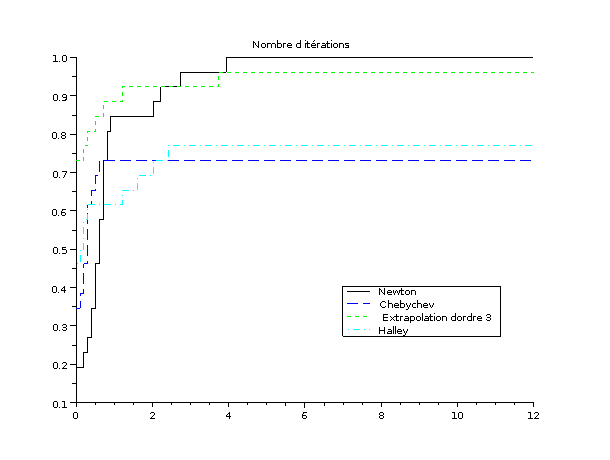
\includegraphics[scale=0.6]{figures/vraiesdirections.png}
\label{fig:vraies}
\end{figure}


L'utilisation de la direction de Newton lorsque celle de Chebychev n'est pas descendante am\'eliore significativement
l'algorithme. En revanche pour Halley, il n'y a presque pas de changement.
\begin{figure}
\caption{Profil des performances : les directions ne sont gard\'ees uniquement s'il s'agit de direction de descente, sinon on 
reprend celle de Newton. Cette fois-ci l'extrapolation d'ordre trois r\'eussit pour tous les probl\`emes.
}\center
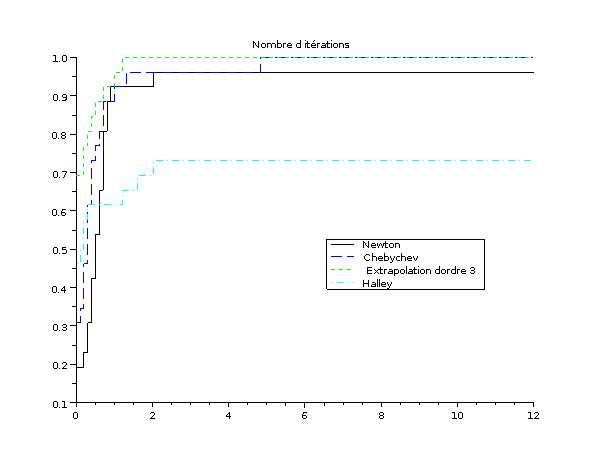
\includegraphics[scale=0.6]{figures/newtonquandpasdescendante.png}
\label{fig:dirnewton}
\end{figure}





% \begin{table}[h]
% 	\begin{center}
% {%\small
%  \footnotesize
% % ---------------------------------------sans l'extrapolation d'ordre 3
% % \begin{tabular}{|l|c|c|c|c|c|c|}
% %   \hline fonction & n & Iter Newton & Iter Cheb & temps Newton & temps Cheby &$\lVert x_{N_f}-x_{C_f}\rVert $\\
% %  \hline
% %    rose& $2$ & $22$ & $16$ & $0.020000$ & $0.017000$ & $0.000000$ \\\hline
% %    froth& $2$ & $8$ & $6$ & $0.007000$ & $0.005000$ & $0.000000$ \\\hline
% %    badscp& $2$ & $999$ & $545$ & $0.878000$ & $0.475000$ & $0.082534$ \\\hline
% %    badscb& $2$ & $9$ & $21$ & $0.009000$ & $0.037000$ & $0.000000$ \\\hline
% %    beale& $2$ & $10$ & $9$ & $0.011000$ & $0.011000$ & $0.000000$ \\\hline
% %    jensam& $2$ & $11$ & $8$ & $0.010000$ & $0.007000$ & $0.000000$ \\\hline
% %    helix& $3$ & $13$ & $14$ & $0.014000$ & $0.022000$ & $0.000000$ \\\hline
% %    bard& $3$ & $13$ & $13$ & $0.013000$ & $0.014000$ & $0.000000$ \\\hline
% %    gauss& $3$ & $3$ & $3$ & $0.003000$ & $0.003000$ & $0.000000$ \\\hline
% %    meyer& $3$ & $163^*$ & $133^*$ & $0.181000$ & $0.177000$ & $0.000000$ \\\hline
% %    gulf& $3$ & $2$ & $2$ & $0.003000$ & $0.004000$ & $Nan$ \\\hline
% %    box& $3$ & $20$ & $135$ & $0.020000$ & $0.132000$ & $66.947050$ \\\hline
% %    sing& $4$ & $22$ & $15$ & $0.020000$ & $0.013000$ & $0.000032$ \\\hline
% %    wood& $4$ & $40$ & $29$ & $0.038000$ & $0.027000$ & $0.000000$ \\\hline
% %    kowosb& $4$ & $9$ & $9$ & $0.009000$ & $0.009000$ & $0.000000$ \\\hline
% %    bd& $4$ & $9$ & $10$ & $0.009000$ & $0.009000$ & $0.000000$ \\\hline
% %    rosex& $10$ & $22$ & $20$ & $0.022000$ & $0.025000$ & $0.000000$ \\\hline
% %    singx& $12$ & $22$ & $17$ & $0.022000$ & $0.017000$ & $0.000134$ \\\hline
% %    pen1& $4$ & $34$ & $25$ & $0.031000$ & $0.023000$ & $0.000000$ \\\hline
% %    vardim& $10$ & $15$ & $11$ & $0.014000$ & $0.010000$ & $0.000000$ \\\hline
% %    trig& $10$ & $10$ & $9$ & $0.012000$ & $0.012000$ & $0.000000$ \\\hline
% %    almost& $10$ & $9$ & $9$ & $0.008000$ & $0.009000$ & $0.214754$ \\\hline
% %    bv& $10$ & $4$ & $3$ & $0.004000$ & $0.003000$ & $0.000000$ \\\hline
% %    ie& $10$ & $4$ & $3$ & $0.004000$ & $0.003000$ & $0.000000$ \\\hline
% %    band& $10$ & $9$ & $8$ & $0.009000$ & $0.008000$ & $0.000000$ \\\hline
% %    cheb& $10$ & $18$ & $20$ & $0.026000$ & $0.031000$ & $0.103538$ \\\hline
% %    \end{tabular}
% 
% \begin{tabular}{|l|c|c|c|c|c|c|c|c|c|}
%   \hline fonction & n & IN & IC & I3 & T N & T C& T E3 &  $\lVert x_{N_f}-x_{C_f}\rVert $ & $\lVert x_{N_f}-x_{3_f}\rVert $ \\
%  \hline
%    rose& $2$ & $22$ & $16$ & $15$ & $0.020$& $0.016$ & $0.019$  & $0.000000$ & $0.000000$ \\\hline
%    froth& $2$ & $8$ & $6$ & $5$ & $0.006$& $0.005$ & $0.005$  & $0.000000$ & $0.000000$ \\\hline
%    badscp& $2$ & $999$ & $545$ & $288$ & $0.874$& $0.477$ & $0.312$ & $0.082534$ & $0.235713$ \\\hline
%    badscb& $2$ & $9$ & $21$ & $18$ & $0.009$& $0.036$ & $0.075$ & $0.000000$ & $0.000000$ \\\hline
%    beale& $2$ & $10$ & $9$ & $8$ & $0.010$& $0.011$ & $0.020$ & $0.000000$ & $0.000000$ \\\hline
%    jensam& $2$ & $11$ & $8$ & $7$ & $0.009$& $0.007$ & $0.008$ & $0.000000$ & $0.000000$ \\\hline
%    helix& $3$ & $13$ & $14$ & $11$ & $0.013$& $0.022$ & $0.017$ & $0.000000$ & $0.000000$ \\\hline
%    bard& $3$ & $13$ & $13$ & $13$ & $0.013$& $0.014$ & $0.017$ & $0.000000$ & $0.000000$ \\\hline
%    gauss& $3$ & $3$ & $3$ & $3$ & $0.002$& $0.002$ & $0.003$ & $0.000000$ & $0.000000$ \\\hline
%    meyer& $3$ & $163^*$ & $133^*$ & $146^*$ & $0.196$& $0.184$ & $0.376$ & $0.000000$ & $0.000000$ \\\hline
%    gulf& $3$ & $2$ & $2$ & $2$ & $0.003$& $0.003$ & $0.010$ & $Nan$ & $Nan$ \\\hline
%    box& $3$ & $20$ & $135$ & $11$ & $0.020$& $0.131$ & $0.017$ & $66.947050$ & $0.000000$ \\\hline
%    sing& $4$ & $22$ & $15$ & $13$ & $0.020$& $0.014$ & $0.014$ & $0.000032$ & $0.000068$ \\\hline
%    wood& $4$ & $40$ & $29$ & $25$ & $0.038$& $0.027$ & $0.030$ & $0.000000$ & $0.000000$ \\\hline
%    kowosb& $4$ & $9$ & $9$ & $9$ & $0.010$& $0.009$ & $0.012$ & $0.000000$ & $0.000000$ \\\hline
%    bd& $4$ & $9$ & $10$ & $11$ & $0.008$& $0.009$ & $0.013$ & $0.000000$ & $0.000000$ \\\hline
%    rosex& $10$ & $22$ & $20$ & $13$ & $0.021$& $0.024$ & $0.023$ & $0.000000$ & $0.000000$ \\\hline
%    singx& $12$ & $22$ & $17$ & $16$ & $0.022$& $0.017$ & $0.020$ & $0.000134$ & $0.000155$ \\\hline
%    pen1& $4$ & $34$ & $25$ & $19$ & $0.031$& $0.023$ & $0.021$ & $0.000000$ & $0.000000$ \\\hline
%    vardim& $10$ & $15$ & $11$ & $10$ & $0.015$& $0.011$ & $0.012$ & $0.000000$ & $0.000000$ \\\hline
%    trig& $10$ & $10$ & $9$ & $9$ & $0.012$& $0.011$ & $0.017$ & $0.000000$ & $0.000000$ \\\hline
%    almost& $10$ & $9$ & $9$ & $12$ & $0.008$& $0.009$ & $0.020$ & $0.214754$ & $0.000000$ \\\hline
%    bv& $10$ & $4$ & $3$ & $3$ & $0.004$& $0.003$ & $0.004$ & $0.000000$ & $0.000000$ \\\hline
%    ie& $10$ & $4$ & $3$ & $3$ & $0.004$& $0.003$ & $0.003$ & $0.000000$ & $0.000000$ \\\hline
%    band& $10$ & $9$ & $8$ & $7$ & $0.009$& $0.008$ & $0.010$ & $0.000000$ & $0.000000$ \\\hline
%    cheb& $10$ & $18$ & $20$ & $13$ & $0.025$& $0.031$ & $0.039$ & $0.103538$ & $0.323658$ \\\hline
% 
% 
%    \end{tabular}
% }
% 	\end{center}
% 	\caption{Tests des m\'ethodes de Newton et Pseudo-Chebychev sur l'ensemble de la librairie MGH avec $x_0$
% relativement proche de la solution : pour Chebychev et l'extrapolation d'ordre 3 la direction n'est gard\'ee que s'il s'agit d'une 
% direction descendante sinon on reprend celle de Newton.}
% 	\label{tab:newton}
% \end{table}


Ensuite, j'ai effectu\'e les mêmes tests mais avec des dimensions plus grandes. Comme point de d\'epart,
j'ai choisi un nombre donn\'e par la fonction random, \`a valeurs comprises entre z\'ero et cent. Sachant que les algorithmes ne sont pas 
globalement convergents, le tableau \ref{tab:111} montre ce fait et en g\'en\'eral, ils ne convergent pas vers le même point.





\begin{table}%[h]
	\begin{center}
{\small
%%%%%%%%%%%%%%%%%%%%%%%%%%%%%%%%%%%%%% Si la m\'ethode de Chebychev n'est pas une direction de Descente 
%on la garde quand meme!!!!!!!!!!!!!!!!!!!!!!!!!!!!!!!!!!!!!!!!!!!
\begin{tabular}{|l|c|c|c|c|c|c|}
  \hline fonction & $n$ & Iter Newton & Iter Cheb & temps Newton & temps Cheby & Norme diff \\
 \hline
   rose& 2 & 77 & 5 & 0.075 & 0.004 & 0.000000 \\\hline
   froth& 2 & 17 & 12 & 0.015 & 0.011 & 0.000000 \\\hline
   badscp& 2 & $19^*$ & 999 & 0.104 & 5.140 & 73081.313391 \\\hline
   badscb& 2 & 18 & 999 & 0.024 & 5.814 & 999915.027828 \\\hline
   beale& 2 & $14^*$ & 999 & 0.074 & 4.536 & 28470.397921 \\\hline
   jensam& 2 & 1 & 1 & 0.001 & 0.002 & Nan \\\hline
   helix& 3 & 14 & 10 & 0.013 & 0.014 & 0.000000 \\\hline
   bard& 3 & 9 & 2 & 0.009 & 0.002 & Nan \\\hline
   gauss& 3 & 1 & 1 & 0.001 & 0.001 & 0.000000 \\\hline
   meyer& 3 & $271^*$ & 999 & 0.302 & 6.159 & 6168.587560 \\\hline
   gulf& 3 & 1 & 1 & 0.001 & 0.001 & 0.000000 \\\hline
   box& 3 & 21 & 6 & 0.021 & 0.016 & Nan \\\hline
   sing& 4 & 26 & 19 & 0.024 & 0.017 & 0.000136 \\\hline
   wood& 4 & 27 & 21 & 0.025 & 0.024 & 0.000000 \\\hline
   kowosb& 4 & 230 & 2 & 0.221 & 0.003 & Nan \\\hline
   bd& 4 & 13 & 12 & 0.013 & 0.011 & 0.000000 \\\hline
   rosex& 10 & 203 & 5 & 0.207 & 0.005 & 0.000000 \\\hline
   singx& 12 & 30 & 24 & 0.030 & 0.023 & 0.000553 \\\hline
   pen1& 4 & 42 & 30 & 0.038 & 0.027 & 0.000000 \\\hline
   vardim& 10 & 26 & 19 & 0.025 & 0.018 & 0.000000 \\\hline
   trig& 10 & 20 & 2 & 0.023 & 0.027 & Nan \\\hline
   almost& 10 & 25 & 28 & 0.078 & 0.297 & Nan \\\hline
   bv& 10 & 22 & 999 & 0.022 & 5.438 & 185.331743 \\\hline
   ie& 10 & 21 & 17 & 0.025 & 0.029 & 0.000000 \\\hline
   band& 10 & 31 & 25 & 0.033 & 0.034 & 0.000000 \\\hline
   cheb& 10 & 167 & 999 & 0.208 & 5.010 & 1.674059 \\\hline
   ie & 100 & 89 & 360 & 2.251 & 11.208 & 0.000000 \\\hline 
   ie& 200 & 177 & 234 & 27.493 & 39.950 & 0.000000 \\\hline
   trig& 100 & 46 & 45 & 0.340 & 0.343 & 0.069866 \\\hline 
   trig& 250 & 61 & 58 & 2.104 & 2.114 & 14217.789748 \\\hline  
   trig& 350 & 61 & 65 & 4.270 & 4.700 & 0.022663 \\\hline  
   bv& 500 & 20 & 16 & 1.172 & 1.016 & 0.0066708 \\\hline
   bv& 1 & 19 & 15 & 5.404 & 4.585 &  0.1489379 \\\hline
   bv& 1500 & 17 & 14 & 10.86 & 9.613 & 12.905217 \\\hline
   bv& 2 & 17 & 13 & 19.097 & 15.863 & 17.806732 \\\hline
\end{tabular}
}
	\end{center}
	\caption{Nombre d'it\'eration des m\'ethodes de Newton et Chebychev mais sur un point initial loin de la 
solution. Les algorithmes convergent rarement au même point.}
	\label{tab:111}
\end{table}





% \begin{table}%[h]
% 	\begin{center}
% {\small
% \begin{tabular}{|l|c|c|c|c|c|c|}
%   \hline fonction & $n$ & Iter Newton & Iter Cheb & temps Newton & temps Cheby & $\lVert x_{N_f}-x_{C_f}\rVert $ \\
%  \hline
% trig& $100 $&$ 6$ &$ 6 $&$ 0.072000 $&$ 0.056000 $&$ 0.000000$ \\\hline %en utilisant le x0
% ie& $300 $&$ 4 $&$ 3 $&$ 1.842000 $& $1.395000 $&$ 0.000000 $\\\hline % en utilisant le x0
% ie& $500 $&$ 4 $& $3 $& $8.047000$ &$ 6.110000 $&$ 0.000000$ \\\hline % en utilisant le x0
% ie& $800 $&$ 4 $& $3 $& $32.200000 $& $24.464000 $&$ 0.000000$ \\\hline % en utilisant le x0
% ie& $300 $&$ 7 $& $5 $& $3.204000$ & $2.324000$ & $0.000000$ \\\hline   % en utilisant le 10* x0
% ie& $500 $&$ 7 $& $5 $& $14.045000 $& $10.163000$ & $0.000000$ \\\hline % en utilisant le 10* x0
% ie& $800 $&$ 7 $&$ 5 $& $56.345000 $& $40.795000 $& $0.000000$ \\\hline % en utilisant le 10* x0
% band& $300$ &$ 9 $& $8$ &$ 0.352000 $& $0.345000 $& $0.000000 $\\\hline  % en utilisant le x0
% band& $500$ &$ 9 $& $8 $& $0.923000 $& $0.884000 $& $0.000000 $\\\hline  % en utilisant le x0
% band& $800$ &$ 9 $& $8 $& $2.566000 $& $2.450000 $& $0.000000 $\\\hline  % en utilisant le x0
% band& $300$ &$ 19$ & $15$ &$ 0.718000$ &$ 0.629000 $& $0.000000$ \\\hline
% \end{tabular}
% }
% 	\end{center}
% 	\caption{Point initial proche suffisamment proche de la solution pour que Chebychev converge : le gain en it\'eration
% n'est pas tr\`es grand. En revanche si la dimension est grande, le gain en temps peut être bon.}
% 	\label{tab:der}
% \end{table}

\begin{table}%[h]
	\begin{center}
{\small
\begin{tabular}{|l|c|c|c|c|c|c|c|c|c|c|}
  \hline fonction & $k*x_0$ & $n$ & IN & IC & I3 & TN & TC & T3 & $\lVert x_{N_f}-x_{C_f}\rVert $ & $\lVert x_{N_f}-x_{3_f}\rVert $  \\
 \hline
bv & 1 & 300 & 2 & 2 & 2 & 0.043 & 0.043 & 0.074 & 0.000042 & 0.000042 \\\hline 
bv & 10 & 300 & 4 & {\bf 3} & 4 & 0.082 & 0.065 & 0.149 & 0.000228 & 0.000308 \\\hline 
bv & 100 & 300 & 13 & {\bf 10 }& 11 & 0.266 & 0.218 & 0.413 & 0.000029 & 0.000267 \\\hline 
bv & 1 & 500 & 7 & 6 & {\bf 4} & 0.407 & 0.375 & 0.433 & 0.000725 & 0.000473 \\\hline 
bv & 10 & 500 & 13 & 13 & 15 & 0.747 & 0.815 & 1.626 & 0.001876 & 0.002417 \\\hline 
bv & 100 & 500 & 23 &{\bf 19} & 21 & 1.323 & 1.193 & 2.289 & 0.001084 & 0.000554 \\\hline 
bv & 1 & 800 & 6 & 5 &{\bf 3} & 1.062 & 0.942 & 0.920 & 0.016409 & 0.141987 \\\hline 
bv & 10 & 800 & 11 & 9 & {\bf 7} & 1.938 & 1.717 & 2.175 & 0.706669 & 0.924390 \\\hline 
bv & 100 & 800 & 21 &{\bf 20} & 17 & 3.720 & 3.841 & 5.325 & 0.798127 & 0.800345 \\\hline
ie & 1 & 300 & 4 & 3 & 3 & 1.834 & 1.398 & 1.468 & 0.000 & 0.000000 \\\hline 
ie & 10 & 300 & 7 & 5 & 5 & 3.205 & 2.330 & 2.474 & 0.000 & 0.000000 \\\hline 
ie & 1 & 500 & 4 & 3 & 3 & 8.044 & 6.105 & 6.348 & 0.000 & 0.000000 \\\hline 
ie & 10 & 500 & 7 & 5 & 5 & 14.054 & 10.155 & 10.556 & 0.000 & 0.000000 \\\hline 
ie & 1 & 800 & 4 & 3 & 3 & 32.521 & 24.463 & 25.169 & 0.000 & 0.000000 \\\hline 
ie & 10 & 800 & 7 & 5 & 5 & 56.313 & 40.456 & 41.555 & 0.000 & 0.000000 \\\hline 
trid & 1 & 300 & 7 & 6 & 6 & 0.152 & 0.129 & 0.204 & 0.000 & 0.000000 \\\hline 
trid & 10 & 300 & 12 & 10 & 10 & 0.246 & 0.215 & 0.344 & 0.000 & 0.000000 \\\hline 
trid & 100 & 300 & 18 & 15 & 14 & 0.369 & 0.325 & 0.482 & 0.000 & 0.000000 \\\hline 
trid & 1 & 500 & 7 & 6 & 6 & 0.397 & 0.366 & 0.579 & 0.000 & 0.000000 \\\hline 
trid & 10 & 500 & 12 & 10 & 10 & 0.673 & 0.613 & 0.967 & 0.000 & 0.000000 \\\hline 
trid & 100 & 500 & 18 & 15 &{\bf 14} & 1.015 & 0.906 & 1.333 & 0.000 & 0.000000 \\\hline 
trid & 1 & 800 & 7 & 6 & 6 & 1.177 & 1.080 & 1.656 & 0.000 & 0.000000 \\\hline 
trid & 10 & 800 & 12 & 10 & 10 & 2.043 & 1.842 & 2.757 & 0.000 & 0.000000 \\\hline 
trid & 100 & 800 & 18 & 15 & 14 & 3.067 & 2.760 & 3.854 & 0.000 & 0.000000 \\\hline 
band & 1 & 300 & 9 & 8 &{\bf 7} & 0.330 & 0.321 & 0.416 & 0.000 & 0.000000 \\\hline 
band & 10 & 300 & 19 & 15 & 15 & 0.695 & 0.608 & 0.894 & 0.000 & 0.000000 \\\hline 
band & 100 & 300 & 29 & 23 & 23 & 1.061 & 0.933 & 1.372 & 0.000 & 0.000000 \\\hline 
band & 1 & 500 & 9 & 8 &{\bf 7} & 0.904 & 0.895 & 1.149 & 0.000 & 0.000000 \\\hline 
band & 10 & 500 & 19 & 15 & 15 & 1.894 & 1.633 & 2.398 & 0.000 & 0.000000 \\\hline 
band & 100 & 500 & 29 & 23 & 23 & 2.892 & 2.508 & 3.680 & 0.000 & 0.000000 \\\hline 
band & 1 & 800 & 9 & 8 &{\bf 7} & 2.538 & 2.408 & 3.018 & 0.000 & 0.000000 \\\hline 
band & 10 & 800 & 19 & 15 & 15 & 5.391 & 4.570 & 6.468 & 0.000 & 0.000000 \\\hline 
band & 100 & 800 & 29 & 23 & 23 & 8.231 & 7.040 & 9.933 & 0.000 & 0.000000 \\\hline 
\end{tabular}
}
	\end{center}
	\caption{En testant avec des dimensions plus grandes. Comme point initial : 1, 10 ou 100 fois $x_0$. Le temps pour 
l'extrapolation d'odre 3 est plus grand car les d\'eriv\'ees sont calcul\'ees \`a partir du gradient fourni et non du mode inverse.}
\label{tab:dimplus}


\end{table}

% \subsection{Avec r\'egion de confiance}
\subsection{Figures qui illustrent les parcours}


\paragraph{Rosenbrock}

Sur les figures \ref{fig:Newton} et \ref{fig:Chebychev}, j'ai trac\'e le chemin qu'emprunte 
l'algorithme de Newton et de Chebychev pour la fonction de Rosenbrock.
On observe bien que sans recherche lin\'eaire, l'algorithme est plus rapide,
cependant la valeur de l'objectif peut augmenter. \`A l'it\'eration $2$, la valeur de l'objectif
 atteint $1411.8$, et si l'algorithme revient vers la solution, c'est {$\scriptscriptstyle\ll$}par chance{$\scriptscriptstyle\gg$} car il n'y a pas de convergence globale.
 Lorsque l'on applique une recherche lin\'eaire, le parcours est mieux contrôl\'e et suit une {$\scriptscriptstyle\ll$}vall\'ee{$\scriptscriptstyle\gg$} o\`u la valeur de la
fonction objectif reste faible.

\begin{figure}
\caption{Newton - La recherche lin\'eaire restreint \`a fournir des it\'er\'es dont la valeur de l'objectif est 
toujours d\'ecroissante tandis que sans recherche, on s'\'eloigne pour converger plus vite.}
\begin{center}
\fbox{
\begin{minipage}[c]{0.6\textwidth}
\beginpgfgraphicnamed{figures/courbe_0}
\endpgfgraphicnamed \\
	  \begin{tabular}{|l|c|c|c|}
	  \hline
	  it\'eration & $x_1$ & $x_2$ &  $f(x)$ \\
	  \hline
	  $0$ & $-1.200000$ & $1.000000$ & $24.200000$ \\
	  $1$ & $-1.175281$ & $1.380674$ & $4.731884$ \\
	  $2$ & $0.763115$ & $-3.175034$ & $1411.845179$ \\
	  $3$ & $0.763430$ & $0.582825$ & $0.055966$ \\
	  $4$ & $0.999995$ & $0.944027$ & $0.313189$ \\
	  $5$ & $0.999996$ & $0.999991$ & $0.000000$ \\
	  $6$ & $1.000000$ & $1.000000$ & $0.000000$ \\
	  \hline
	  \end{tabular}\\
\end{minipage}
}
\end{center}
\label{fig:Newton}
\end{figure}

% \vspace{1cm}


% \begin{table}%[h]
% 	\begin{center}
% 	  \begin{tabular}{|l|c|c|c|}
% 	  \hline
% 	  it\'eration & $x_1$ & $x_2$ &  $f(x)$ \\
% 	  \hline
% 	  $0$ & $-1.200000$ & $1.000000$ & $24.200000$ \\
% 	  $1$ & $-1.175281$ & $1.380674$ & $4.731884$ \\
% 	  $2$ & $0.763115$ & $-3.175034$ & $1411.845179$ \\
% 	  $3$ & $0.763430$ & $0.582825$ & $0.055966$ \\
% 	  $4$ & $0.999995$ & $0.944027$ & $0.313189$ \\
% 	  $5$ & $0.999996$ & $0.999991$ & $0.000000$ \\
% 	  $6$ & $1.000000$ & $1.000000$ & $0.000000$ \\
% 	  \hline
% 	  \end{tabular}\\
% 	\end{center}
% 	\caption{It\'er\'es de la m\'ethode de Newton sur la fonction Rosenbrock sans recherche lin\'eaire.}
% 	\label{tab:newton}
% \end{table}





\begin{figure}
\caption{Chebychev - La direction de Chebychev est meilleure sur l'exemple, cependant qu'une seule it\'eration n'est gagn\'ee}
\begin{center}
\fbox{
\begin{minipage}[c]{0.6\textwidth}
% \begin{center}
\beginpgfgraphicnamed{figures/courbe_1}
\endpgfgraphicnamed \\
	\begin{tabular}{|l|c|c|c|}
	\hline
	it\'eration & $x_1$ & $x_2$ &  $f(x)$ \\
	\hline
	$0$ & $-1.200000$ & $1.000000$ & $24.200000$ \\
	$1$ & $-1.150840$ & $1.322626$ & $4.626437$ \\
	$2$ & $0.848588$ & $-0.780668$ & $225.254139$ \\
	$3$ & $0.849592$ & $0.721806$ & $0.022623$ \\
	$4$ & $1.000000$ & $0.999993$ & $0.000000$ \\
	$5$ & $1.000000$ & $1.000000$ & $0.000000$ \\
	\hline
	\end{tabular}
%\end{center}
\end{minipage}
}
\end{center}
% \beginpgfgraphicnamed{figures/courbe_1}
% \endpgfgraphicnamed

\label{fig:Chebychev}
\end{figure}


% \begin{table}%[h]
% 	\begin{center}
% 	\begin{tabular}{|l|c|c|c|}
% 	\hline
% 	it\'eration & $x_1$ & $x_2$ &  $f(x)$ \\
% 	\hline
% 	$0$ & $-1.200000$ & $1.000000$ & $24.200000$ \\
% 	$1$ & $-1.150840$ & $1.322626$ & $4.626437$ \\
% 	$2$ & $0.848588$ & $-0.780668$ & $225.254139$ \\
% 	$3$ & $0.849592$ & $0.721806$ & $0.022623$ \\
% 	$4$ & $1.000000$ & $0.999993$ & $0.000000$ \\
% 	$5$ & $1.000000$ & $1.000000$ & $0.000000$ \\
% 	\hline
% 	\end{tabular}
% 	\end{center}
% 	\caption{It\'er\'es de la m\'ethode de Chebychev sur la fonction Rosenbrock}
% 	\label{tab:chebychev}
% \end{table}




\begin{figure}%[!h]
\caption{Ordre sup\'erieur : la direction s'\'eloigne encore moins de la vall\'ee que les proc\'ed\'es de Newton ou Chebychev.}
\begin{center}
\fbox{
\begin{minipage}[c]{0.7\textwidth}
\beginpgfgraphicnamed{figures/courbe_2}
\endpgfgraphicnamed \\
	\begin{tabular}{|l|c|c|c|}
	\hline
	it\'eration & $x_1$ & $x_2$ &  $f(x)$ \\
	\hline
	$0$ & $-1.200000$ & $1.000000$ & $24.200000$ \\
	$1$ & $-1.126673$ & $1.265834$ & $4.524003$ \\
	$2$ & $0.847210$ & $-0.350714$ & $114.187943$ \\
	$3$ & $0.849335$ & $0.721366$ & $0.022700$ \\
	$4$ & $1.000000$ & $1.000000$ & $0.000000$ \\
	$5$ & $1.000000$ & $1.000000$ & $0.000000$ \\
	\hline
	\end{tabular}\\
\end{minipage}
}
\end{center}
\label{fig:sup}
\end{figure}





% \begin{table}%[!h]
% 	\begin{center}
% 	\begin{tabular}{|l|c|c|c|}
% 	\hline
% 	it\'eration & $x_1$ & $x_2$ &  $f(x)$ \\
% 	\hline
% 	$0$ & $-1.200000$ & $1.000000$ & $24.200000$ \\
% 	$1$ & $-1.126673$ & $1.265834$ & $4.524003$ \\
% 	$2$ & $0.847210$ & $-0.350714$ & $114.187943$ \\
% 	$3$ & $0.849335$ & $0.721366$ & $0.022700$ \\
% 	$4$ & $1.000000$ & $1.000000$ & $0.000000$ \\
% 	$5$ & $1.000000$ & $1.000000$ & $0.000000$ \\
% 	\hline
% 	\end{tabular}\\
% 	\end{center}
% 	\caption{It\'er\'es de la m\'ethode d'extrapolation d'ordre 3 sur la fonction Rosenbrock}
% 	\label{tab:extra3}
% \end{table}


% \cite{historical}\cite{cauchy}



